\documentclass[ignorenonframetext,]{beamer}

%Set up notes
\setbeamertemplate{note page}[plain]
\setbeameroption{hide notes}

\usepackage{amssymb,amsmath}
\usepackage{ifxetex,ifluatex}
\usepackage{fixltx2e} % provides \textsubscript
\usepackage{tikz}
\usepackage{tikz-qtree}
\usepackage{pdfpages} %include beamer pdf slides from other presentations
\ifxetex
  \usepackage{fontspec,xltxtra,xunicode}
  \defaultfontfeatures{Mapping=tex-text,Scale=MatchLowercase}
\else
  \ifluatex
    \usepackage{fontspec}
    \defaultfontfeatures{Mapping=tex-text,Scale=MatchLowercase}
  \else
    \usepackage[utf8]{inputenc}
  \fi
\fi

% Comment these out if you don't want a slide with just the
% part/section/subsection/subsubsection title:
\AtBeginPart{
  \let\insertpartnumber\relax
  \let\partname\relax
  \frame{\partpage}
}
\AtBeginSection{
  \let\insertsectionnumber\relax
  \let\sectionname\relax
  \frame{\sectionpage}
}
\AtBeginSubsection{
  \let\insertsubsectionnumber\relax
  \let\subsectionname\relax
  \frame{\subsectionpage}
}

\setlength{\parindent}{0pt}
\setlength{\parskip}{6pt plus 2pt minus 1pt}
\setlength{\emergencystretch}{3em}  % prevent overfull lines
\setcounter{secnumdepth}{0}

\title{The Ricardian (Comparative Advantage) Model of International Trade (\emph{MODIFIED})}
\author{Instructor: David Jinkins}
\date{Date: Sept. 4, 2014}

\begin{document}
\frame{\titlepage}

\begin{frame}
\begin{itemize}
\itemsep1pt\parskip0pt\parsep0pt
\item
  Last time 

  \begin{itemize}
  \itemsep1pt\parskip0pt\parsep0pt
  \item You should care about international economics because:
      \begin{enumerate}
          \item Denmark is small, world is large
          \item Lots of popular misconceptions
          \item Still many puzzles and counter-intuitive ideas
      \end{enumerate}
  \item Gravity model:
      \begin{enumerate}
          \item Trade proportional to product of partner sizes 
          \item Trade falls with distance, geographic and cultural 
      \end{enumerate}
  \item Gravity model for some reason describes trade flows well
  \item Distance costs still seem unreasonably large 
  \end{itemize}
\end{itemize}

\end{frame}

\begin{frame}

\begin{itemize}
  \item Last time: Ricardo
  \item Basic model:
  \begin{enumerate}
    \item The parable of my RA's
    \item Who makes what?
  \end{enumerate}
  \item Analysis of model results 
  \begin{enumerate}
    \item Specialization and gains 
    \item Wages and productivity 
    \item Extensions
  \end{enumerate}
\end{itemize}

\end{frame}

\begin{frame}

\begin{itemize}
\itemsep1pt\parskip0pt\parsep0pt
\item
  Today: More Gravity and Ricardo
  \begin{itemize}
        \item Gravity
        \begin{enumerate}
            \item A puzzle
            \item Where does gravity come from?
        \end{enumerate}
        \item Ricardo
        \begin{itemize}
            \item Review
            \item Ricardo with many goods 
            \item Ricardo with factor movement 
            \item Confronting the data 
            \item Common misunderstandings
            \item Limitations of Ricardo
            \item If time: a numerical example
        \end{itemize}
  \end{itemize}
\end{itemize}

\end{frame}

\begin{frame}

    Section 1: Gravity again 

\end{frame}

\begin{frame}{The gravity equation}
    
    \begin{itemize}
        \item Gravity equation (gravity):
        \begin{equation*}
            F_{ij} = g \frac{M_i M_j}{d_{ij}^2}
        \end{equation*}
        \item Gravity equation (trade):
        \begin{equation*}
            X_{ij} = g \frac{\mbox{GDP}_i \mbox{GDP}_j}{d_{ij}^\theta}
        \end{equation*}
        \item typically $\theta \approx 1$
        \item Empirical fact first observed by Tinbergen in 1960's.
    \end{itemize}

\end{frame}

\begin{frame}{Puzzle}
    
    \begin{itemize}
        \item Gravity equation (trade):
        \begin{equation*}
            X_{ij} = g \frac{\mbox{GDP}_i \mbox{GDP}_j}{d_{ij}^\theta}
        \end{equation*}
        \item typically $\theta \approx 1$
    \end{itemize}

    \begin{itemize}
        \item What happens to trade if the economy of every country doubles?
    \end{itemize}

\end{frame}

\begin{frame}

    \begin{itemize}
        \item Denmark's export to GDP ratio is about a third
        \item Recently world GDP doubles every 30 years
        \item According to gravity, what will Denmark's export to GDP ratio look like in 60 years? 
    \end{itemize}
    \begin{itemize}
        \item Theoretical problem with the gravity model
        \item Why not in physics? 
    \end{itemize}

\end{frame}

\begin{frame}{Where does economic gravity come from?}

    \begin{itemize}
        \item \dots and what is wrong with it? 
        \item Let's sketch one possible derivation.
    \end{itemize}

\end{frame}

\begin{frame}{Where does economic gravity come from?}

    \begin{itemize}
        \item Takeaway 
        \begin{itemize}
            \item Theoretically grounded gravity slightly different:
            \item Gravity equation (theoretically grounded):
            \begin{equation*}
                X_{ij} = R_j \frac{\mbox{GDP}_i \mbox{GDP}_j}{d_{ij}^\theta}
            \end{equation*}
        \end{itemize}
        \item Remoteness term is important
        \begin{itemize}
            \item Portugal-Austria about the same distance as Australia-New Zealand
            \item GDP products also about the same 
            \item But New Zealand-Australia trade nine times higher!
        \end{itemize}
    \end{itemize}

\end{frame}

\begin{frame}
    
    \begin{itemize}
        \item Gravity equation (theoretically grounded):
        \begin{equation*}
            X_{ij} = R_j \frac{\mbox{GDP}_i \mbox{GDP}_j}{d_{ij}^\theta}
        \end{equation*}
        \item We learned that if $\theta = 1$, exports halve if distance doubles.
        \item What would happen to Portugal-Austrian trade if we moved Portugal twice as far away into the Atlantic Ocean?  
    \end{itemize}

\end{frame}

\begin{frame}

    \begin{itemize}
        \item Some recent gravity research:
        \item Head, Meier, and Reis, The Erosion of Colonial Trade Linkages, Journal of International Economics, 2010
    \end{itemize}

\end{frame}

\begin{frame}

    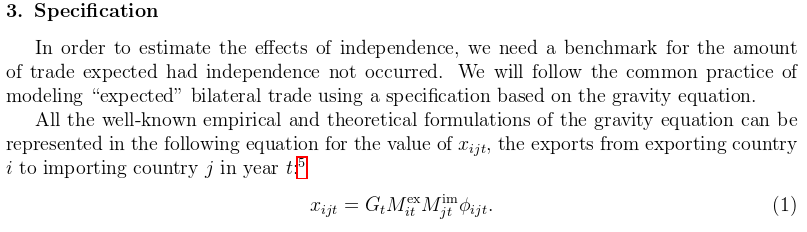
\includegraphics[scale=0.30]{gravity_in_research.png}

\end{frame}

\begin{frame}

    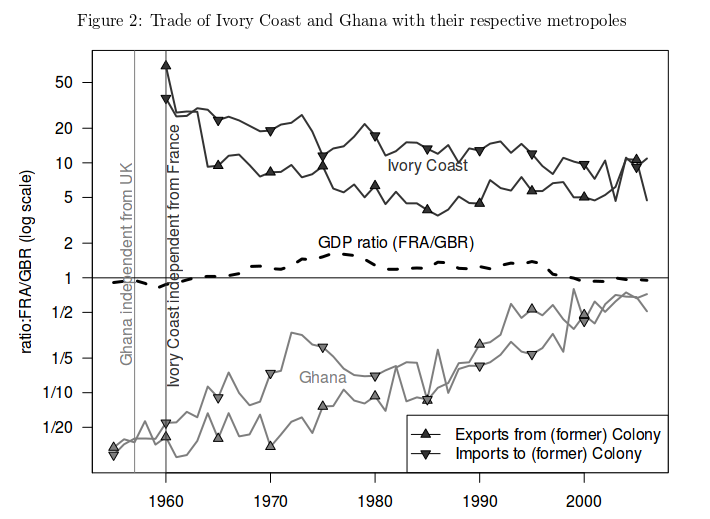
\includegraphics[scale=0.30]{erosion_of_colonial_trade.png}

\end{frame}

\begin{frame}

    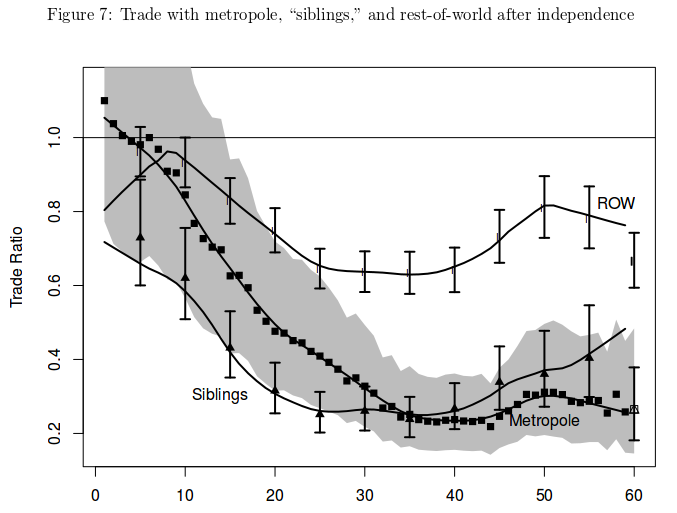
\includegraphics[scale=0.30]{siblings_trade.png}

\end{frame}

\begin{frame}

    \begin{itemize}
        \item End gravity section
        \item Begin Ricardo review
    \end{itemize}

\end{frame}

\begin{frame}{The Ricardian model}

    \begin{itemize}
        \item Reason for trade 'technology' differences {\footnotesize other models: resource endowments, increasing returns to scale}
        \item Countries \emph{can} make more by specializing (to some degree)
        \item Countries \emph{will} specialize if allowed to trade freely
        \item Free trade weakly benefits all participants (relative to autarchy) \emph{even if some countries are terrible at everything.}
    \end{itemize}

\end{frame}

\begin{frame}{The RA Parable}

    \begin{center}
        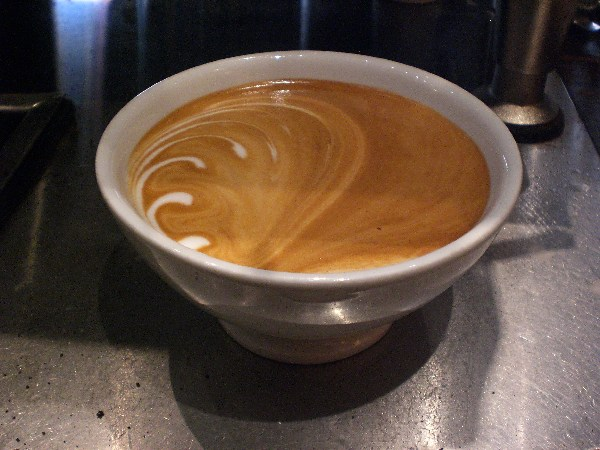
\includegraphics[scale=0.4]{latte.jpg}
    \end{center}

    {\tiny source: http://en.wikipedia.org/wiki/Latte}

\end{frame}

\begin{frame}{The RA Parable}

    \begin{itemize}
        \item What have we learned:
        \begin{enumerate}
            \item We can produce more by specializing
            \item Even terrible partner can help, by doing what he is less terrible at.
        \end{enumerate}
        \item It is \emph{possible} to increase production through specialization
        \item Will this happen in the free market?
        \item If so, which country gains from free trade?
    \end{itemize}

\end{frame}

\begin{frame}{The Ricardian Model}

    \begin{itemize}
        \item Simplest model able to examine these issues.
        \item Environment:
        \begin{itemize}
            \item Two countries
            \begin{enumerate}
                \item Home has $L$ hours of labor
                \item Foreign has $L^*$ hours of labor
            \end{enumerate}
            \item Two goods - wine and cheese
        \end{itemize}
    \end{itemize}

\end{frame}

\begin{frame}{Production}

    \begin{itemize}
        \item Only input to wine and cheese production is labor
        \item Competitive markets, free entry of firms, no profits
        \item Home
        \begin{itemize}
            \item One unit of wine takes $a_w$ hours
            \item One unit of cheese takes $a_c$ hours
        \end{itemize}
        \item Foreign
        \begin{itemize}
            \item One unit of wine takes $a_w^*$ hours
            \item One unit of cheese takes $a_c^*$ hours
        \end{itemize}
        \item Jargon: differences in production technology
    \end{itemize}

\end{frame}

\frame[plain]{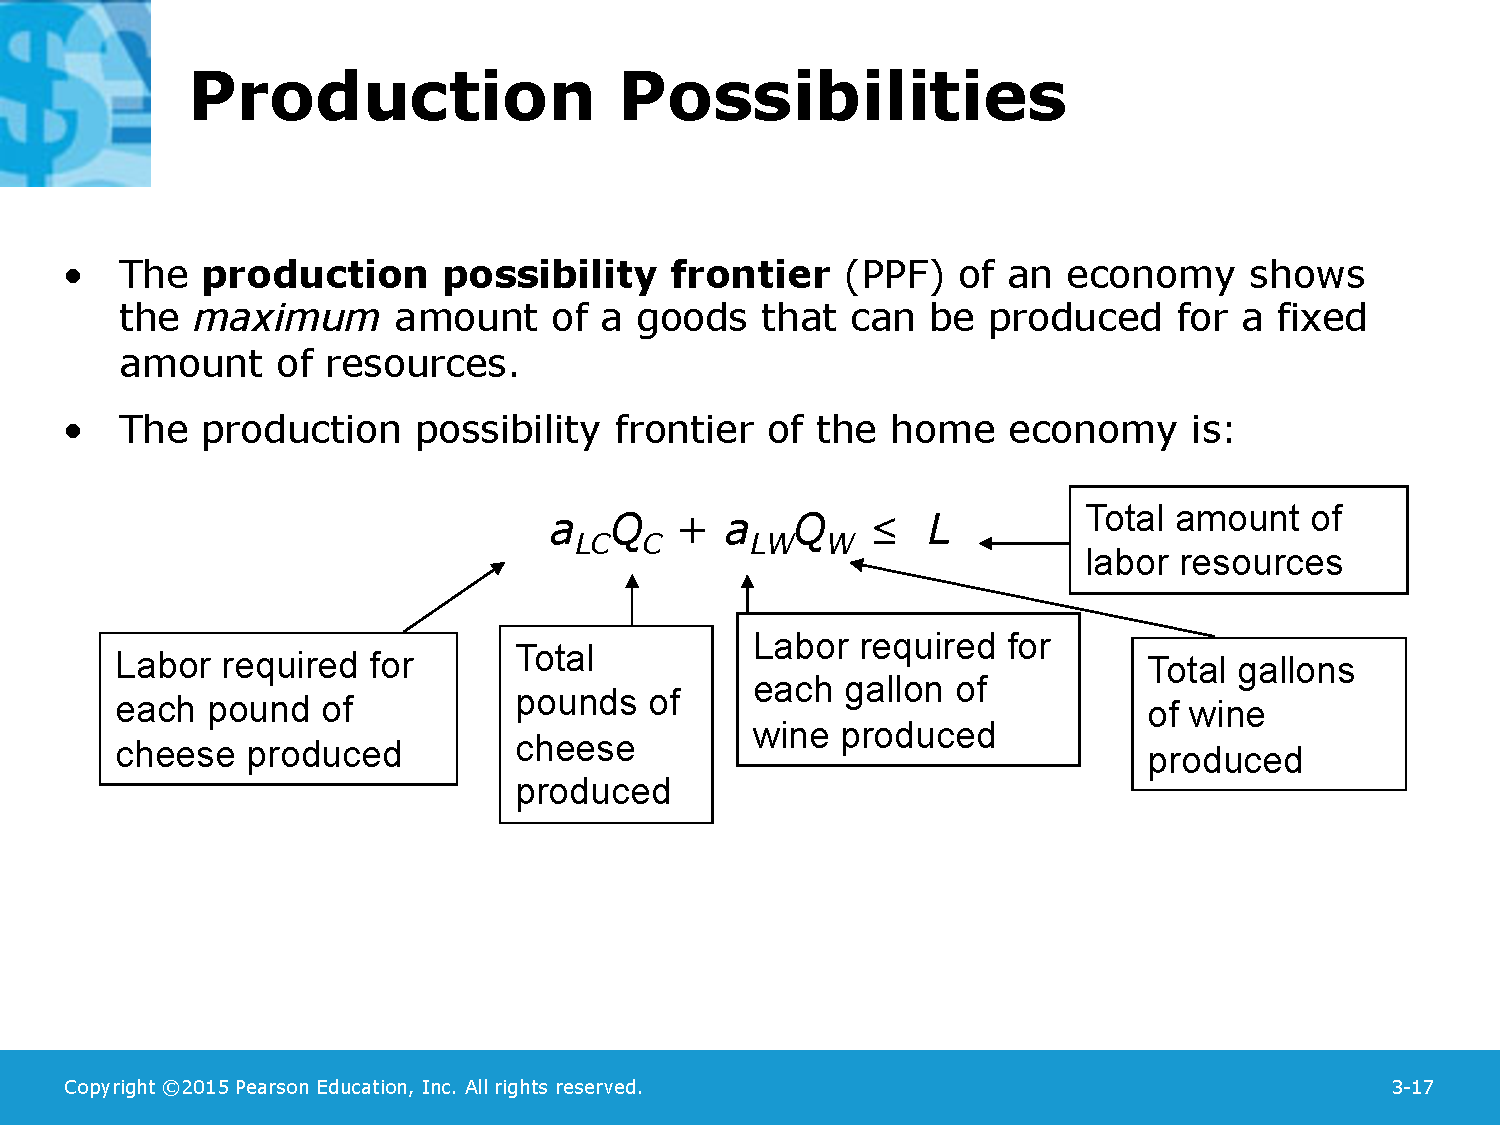
\includegraphics[page=1,width=\textwidth]{PPF_pearson_snippet.pdf}}

\begin{frame}{Comparative Advantage}

    \begin{itemize}
        \item Assume $\frac{a_c}{a_w} < \frac{a_c^*}{a_w^*}$
        \item AKA Home has a comparative advantage in cheese 
        \item Don't know if $a_c$ is less or greater than $a_c^*$
        \item Absolute advantage not important for analysis
    \end{itemize}

\end{frame}

\begin{frame}{Actions}

    \begin{itemize}
        \item Supply
        \begin{itemize}
            \item Workers freely mobile between wine and cheese
            \item Work in sector with higher wages 
            \item Cannot move between countries 
        \end{itemize}
        \item Demand
        \begin{itemize}
            \item Consumers consume wine and cheese to maximize utility
            \item Constrained by labor income
            \item If price of one good rises, substitute other good
            \item Free Trade: Can buy goods produced anywhere
        \end{itemize}
    \end{itemize}

\end{frame}

\begin{frame}{Equilibrium conditions}

    \begin{itemize}
        \item Prices, wages, good and labor quantities such that:
        \begin{enumerate}
            \item Good quantities solve representative consumer's maximization problem given prices and wages 
            \item Labor quantities satisfy firm's problem given prices and wages
            \item International goods markets clear
            \item Domestic labor markets clear
            \item Trade is balanced
        \end{enumerate}
        \item We will summarize all these conditions with a (relative) supply and demand chart.
    \end{itemize}

\end{frame}

\begin{frame}{Detour: Some immediate implications}

    \begin{itemize}

        \item Autarchy wage is the value of a worker's product.  Why?
            \begin{equation*}
                w = \frac{P_c}{a_c} = \frac{P_w}{a_w}
            \end{equation*}
        \item Krugman et al. writes it this way:
            \begin{equation*}
                \frac{P_c}{P_w} = \frac{a_c}{a_w}
            \end{equation*}
        \item What happens if $P_c$ goes up a tiny bit?

    \end{itemize}

\end{frame}

\begin{frame}{Graphical analysis of equilibrium}

    \begin{itemize}
        \item Krugman et. al being a bit tricky with demand\dots
    \end{itemize}

\end{frame}

\begin{frame}

    Section 2: Analysis of model results
\end{frame}

\begin{frame}

    \begin{itemize}
        \item What was the point of all this work?
        \item Question 1: Does trade cause specialization?
        \item Question 2: Does trade make people better off?  In which country?
            \begin{equation*}
                \frac{a_c}{a_w} \leq \frac{P^e_c}{P^e_w} \leq \frac{a_c^*}{a_w^*}
            \end{equation*} 
    \end{itemize}

\end{frame}

\begin{frame}{Gains from trade}

    \begin{itemize}
        \item How much wine can home get with one hour of labor?
        \item Autarchy: $\frac{1}{a_w} $
        \item Trade: $\frac{P^e_c}{P^e_w}\frac{1}{a_c}$
        \item Ricardian equilibrium: 

            \begin{equation*}
                \frac{P^e_c}{P^e_w}\frac{1}{a_c} \geq \frac{P^a_c}{P^a_w}\frac{1}{a_c} = \frac{a_c}{a_w}\frac{1}{a_c} = \frac{1}{a_w}
            \end{equation*}
    \end{itemize}

\end{frame}

\begin{frame}{Gains from trade}

    \begin{itemize}
        \item Textbook: Expansion in consumption possibilities frontier 
        \item What is the slope of the consumption possibilities frontier under free trade?
    \end{itemize}

\end{frame}

\begin{frame}{Relative wages}

    \begin{itemize}
        \item All countries weakly gain from trade
        \item Does not mean that wages are the same across countries 
    \end{itemize}

    \begin{itemize}
        \item $w = \frac{P^e_c}{a_c}$
        \item $w^* = \frac{P^e_w}{a_w^*}$
        \item $\frac{a_w^*}{a_w} \leq \frac{w}{w^*} \leq \frac{a_c^*}{a_c}$
    \end{itemize}

\end{frame}

\begin{frame}{Typical: low productivity, low wage}

    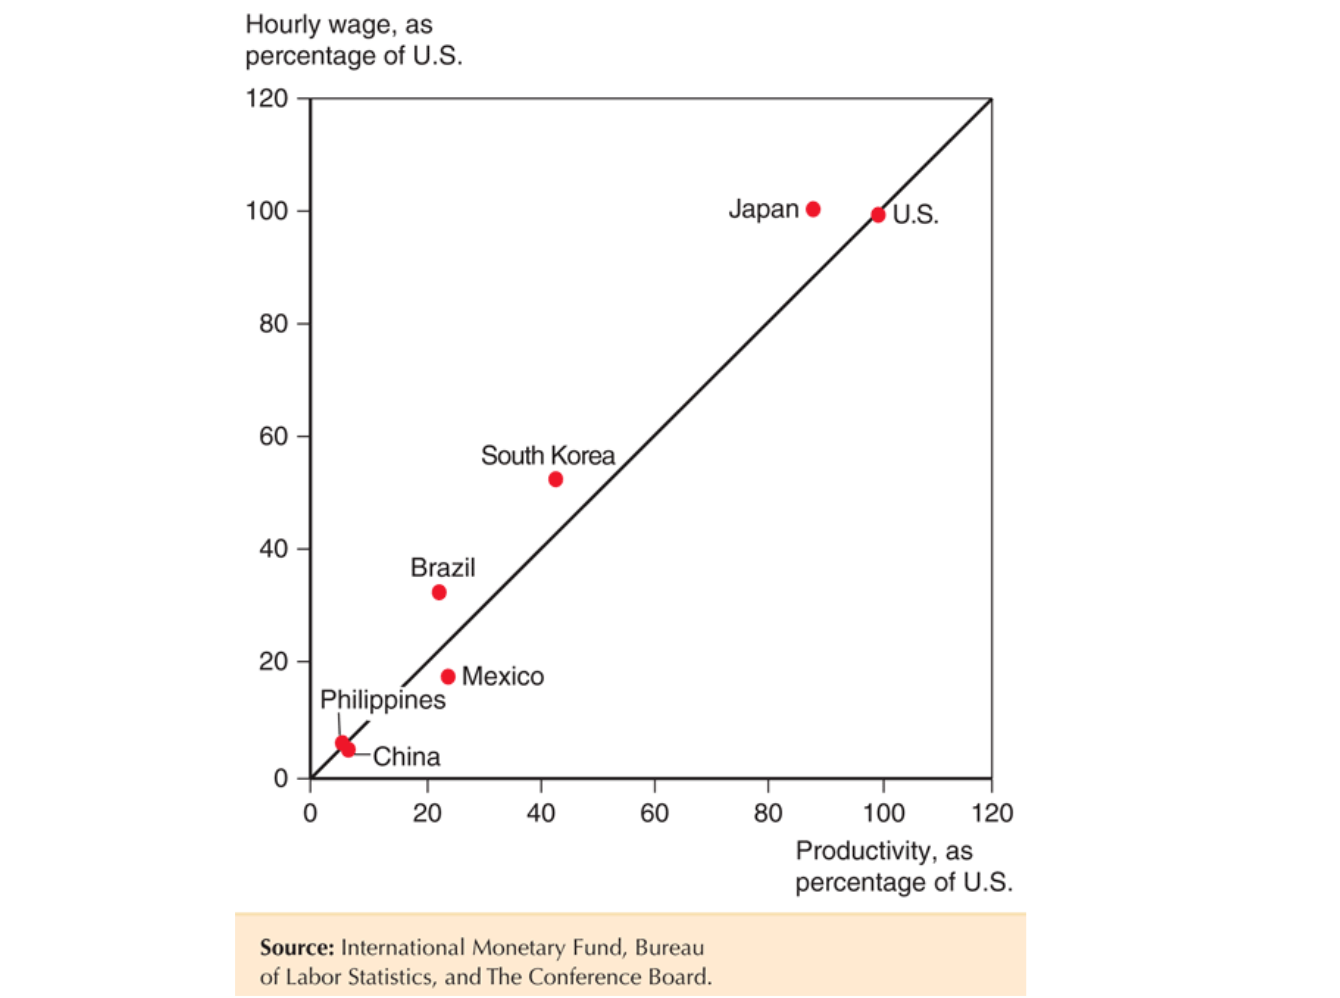
\includegraphics[scale=0.25]{low_prod_low_wage.png}

\end{frame}

\begin{frame}{Some additional observations}

    \begin{itemize}
        \item The more different comparative advantage, the more likely mutual gains
        \item Countries with bad technology are more likely to gain from trade (developing countries!)
    \end{itemize}

\end{frame}

\begin{frame}{Ricardo with many goods}

    \begin{itemize}
        \item Analysis similar
        \item ``Derived demand'': relative demand for labor rather than goods 
        \item False prediction: at most one good produced in both countries
    \end{itemize}

\end{frame}

\begin{frame}{Ricardo with many goods}

    \begin{itemize}
        \item Analysis similar
        \item ``Derived demand'': relative demand for labor rather than goods 
        \item False prediction: at most one good produced in both countries
    \end{itemize}

\end{frame}

\begin{frame}{Ricardo with freely mobile labor}

    \begin{itemize}
        \item First two-good model
        \begin{enumerate}
            \item If one country has absolute advantage in both goods, where will people live?
            \item If each country has absolute advantage in one good, where will people live?
            \item Is it comparative or absolute advantage that determines trade patterns?
            \item What equilibrium condition are we adding to the model? 
        \end{enumerate}
        \item Many good model: 
        \begin{enumerate}
            \item Can we compare absolute advantage as we did in the two-country case?
            \item How can we use the derived demand chart to find the equilibrium here?
        \end{enumerate}
    \end{itemize}

\end{frame}

\begin{frame}{Trade costs and non-tradables}

    \begin{itemize}
        \item High trade costs, countries both produce weak comparative advantage goods
        \item Non-tradables are goods with very high trade costs 
        \item Still specialize in goods with largest comparative advantage
    \end{itemize}

\end{frame}

\begin{frame}{Recent extensions to the Ricardian model}

    \begin{itemize}
        \item Extension to many goods-easy
        \item Extension to many countries-difficult
        \item Eaton and Kortum (2002) linked a Ricardian model to a gravity equation 
        \item Methodology has united and revolutionized economic research in trade
    \end{itemize}

\end{frame}

\begin{frame}
    Section 3: Odds and ends 
    \begin{itemize}
        \item Confronting the data
        \item Common misconceptions
        \item Limitations of Ricardo
    \end{itemize}
\end{frame}

\begin{frame}{Empirical results on Ricardo}

    \begin{itemize}
        \item Ricardian model is simple, world is complex
        \begin{enumerate}
            \item More than two countries
            \item More than two goods 
            \item In particular, more than one input in production
        \end{enumerate}
        \item Takeaway: the empirical 'tests' of Ricardo are somewhat ad-hoc and atheoretical
        \item Basic prediction -- comparative advantage should correspond to trade flows 
        \item Countries should export goods for which their relative productivity is high 
    \end{itemize}

\end{frame}

\begin{frame}{Side note: Productivity}

    \begin{itemize}
        \item Plastic, electricity, eletrical components come to the gate of the iPhone factory
        \item Productivity growth -- we can use exactly the same input materials and produce more iPhones
        \item Productivity growth is what makes us rich
        \item For our purposes, (labor) productivity is: 
        \begin{equation*}
            \frac{\mbox{factory output value} - \mbox{factory input material value}}{\mbox{number of employees}}
        \end{equation*}
    \end{itemize}

\end{frame}

\begin{frame}{China and Bangladesh}

    \begin{itemize}
        \item Prediction: Bangladesh \emph{relatively} productive in textiles 
    \end{itemize}
    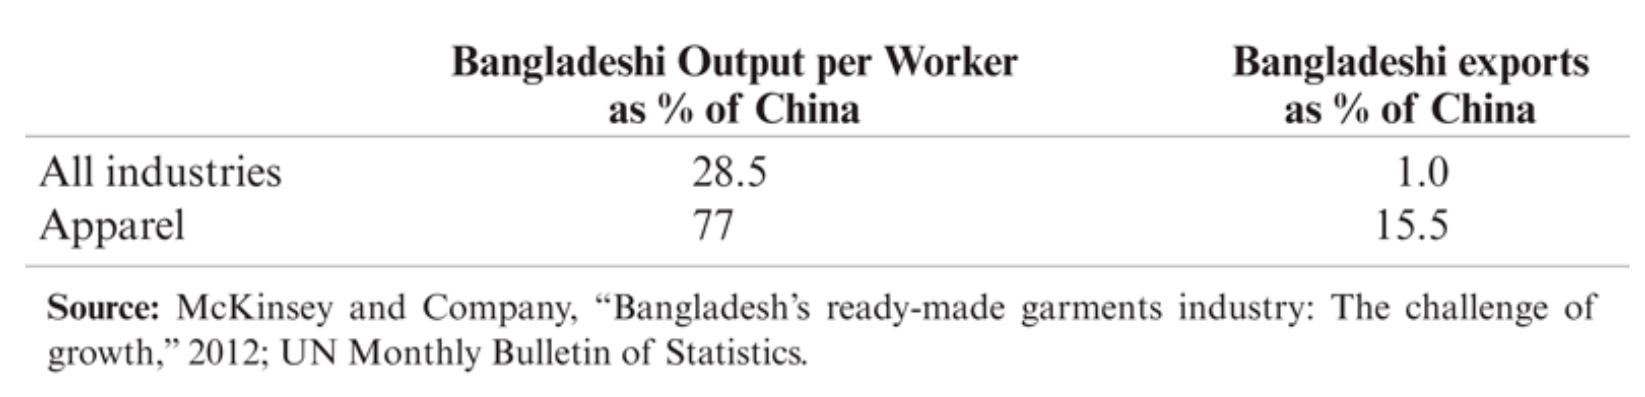
\includegraphics[scale=0.15]{bangladesh_china_cpa.png}

\end{frame}

\begin{frame}{US and UK}

    \begin{itemize}
        \item Prediction: US will export relatively more in industries in which it is relatively productive
    \end{itemize}
    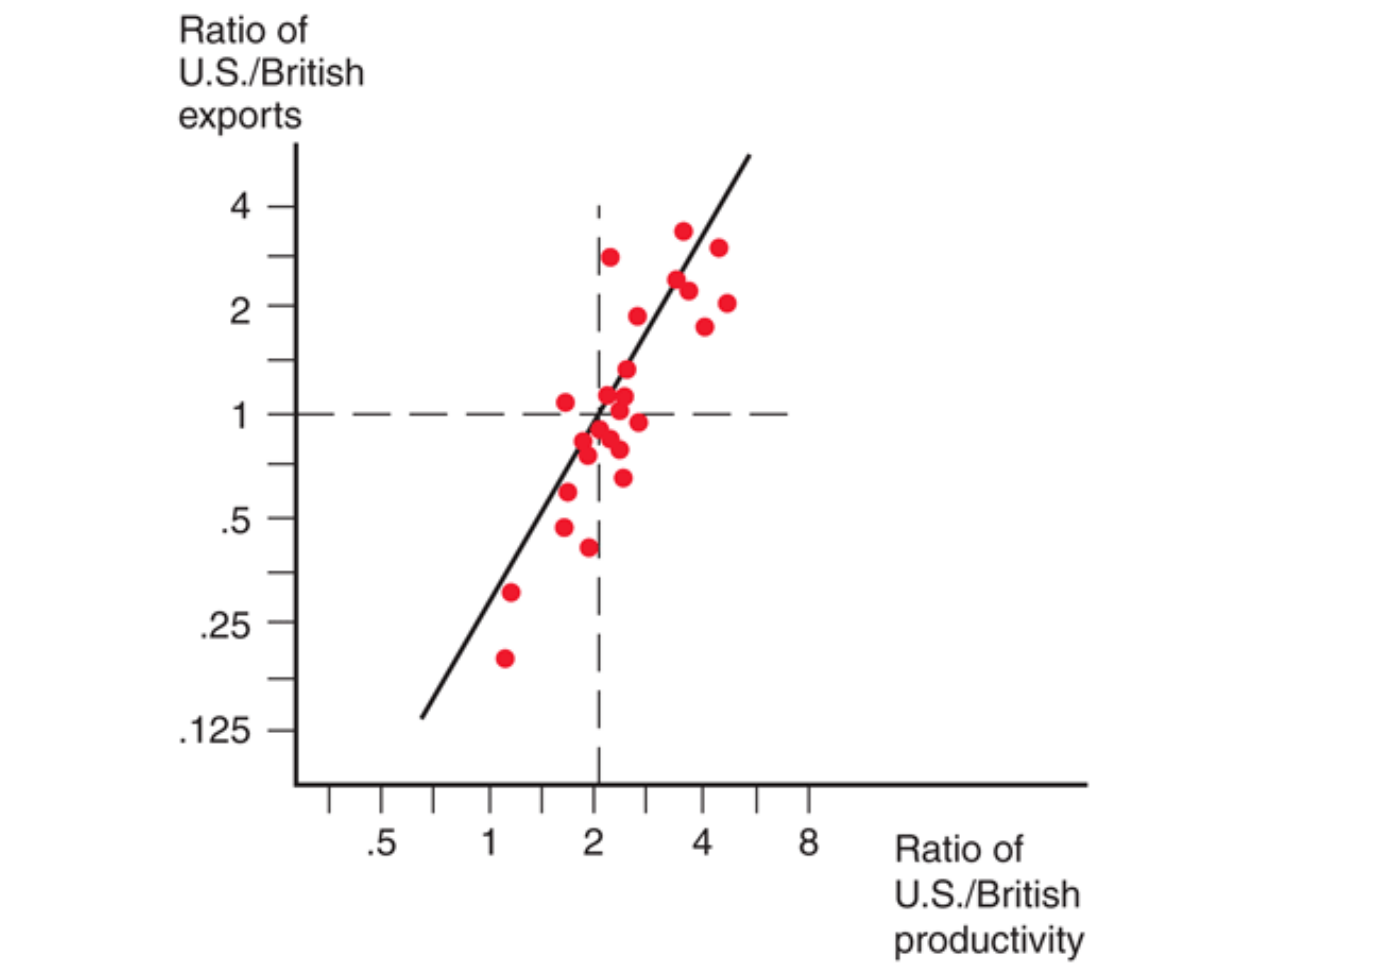
\includegraphics[scale=0.20]{brit_us_exports.png}

\end{frame}

\begin{frame}{Popular misconceptions}

    \begin{enumerate}
        \item Trade only helps countries that are more productive than other countries
        \begin{itemize}
            \item Trade helps poor countries avoid wasting resources in unproductive industries
        \end{itemize}
        \item Trade with low wage countries hurts high wage countries (\emph{pauper labor} argument)
        \begin{itemize}
        \item Trade allows consumers in rich countries to buy goods more cheaply
        \item Trade may, however, hurt some in rich countries -- next class
        \end{itemize}
        \item Trade hurts poor countries because low wages are needed to allow exports
        \begin{itemize}
            \item Too bad that people have low wages, but what is the alternative?
            \item Detour: Same reply to sweatshop protesters
        \end{itemize}
    \end{enumerate}

\end{frame}

\begin{frame}{Limitation of Ricardo}

    \begin{itemize}
        \item Original Ricardo example(1819): Portugal and the UK, clothes and wine.
        \item Portugal better at both, still gains from trading with UK.
        \item Joan Robinson's cheap shot: 
        \item Portugal \emph{did} open up to trade with the UK at this time -- experienced a century of decline!
    \end{itemize}

\end{frame}

\begin{frame}{Limitation of Ricardo}

    \begin{itemize}
        \item Begs the question: why do countries have different technology?
        \item Can't move the weather -- Denmark grows corn and Jordan dates.
        \item Why can't we just manufacture everything everywhere and avoid trade costs?
    \end{itemize}

\end{frame}

\begin{frame}{Institutions}

    \begin{itemize}
        \item Due to the legacy of history or maybe culture, different:
        \begin{itemize}
            \item ease of contract enforcement
            \item ease of accessing credit 
            \item level of trust 
            \item ease of hiring and firing employees 
            \item crime 
            \item government regulations and bureaucracy 
        \end{itemize}
        \item One way to explain link between location and productivity
    \end{itemize}

\end{frame}

\begin{frame}{Summary}

    \begin{itemize}
        \item Ricardian model
        \begin{itemize}
            \item Reason for trade: technology
            \item Mechanism: Reducing production using poor technologies
        \end{itemize}
        \item Some results
        \begin{itemize}
            \item Comparative, not absolute, advantage determines trade flows 
            \item Careful equilibrium analysis -- every country (weakly) gains from free trade
            \item Gains more likely for smaller, poorer countries with very large comparative advantage
            \item Wages can be very different across countries in equilibrium
        \end{itemize}
        \item Confronting the data
        \begin{itemize}
            \item Evidence that Ricardo is part, but not all, of the story
            \item People within a country are not homogenous
        \end{itemize}
    \end{itemize}

\end{frame}

\begin{frame}

    \begin{itemize}
        \item Next time:
            \begin{itemize}
                \item Who gains and who loses if trade is allowed?
                \item The specific-factor model
                \item Explains why pro-trade policies are often unpopular politically
            \end{itemize}
    \end{itemize}

\end{frame}

\frame[plain]{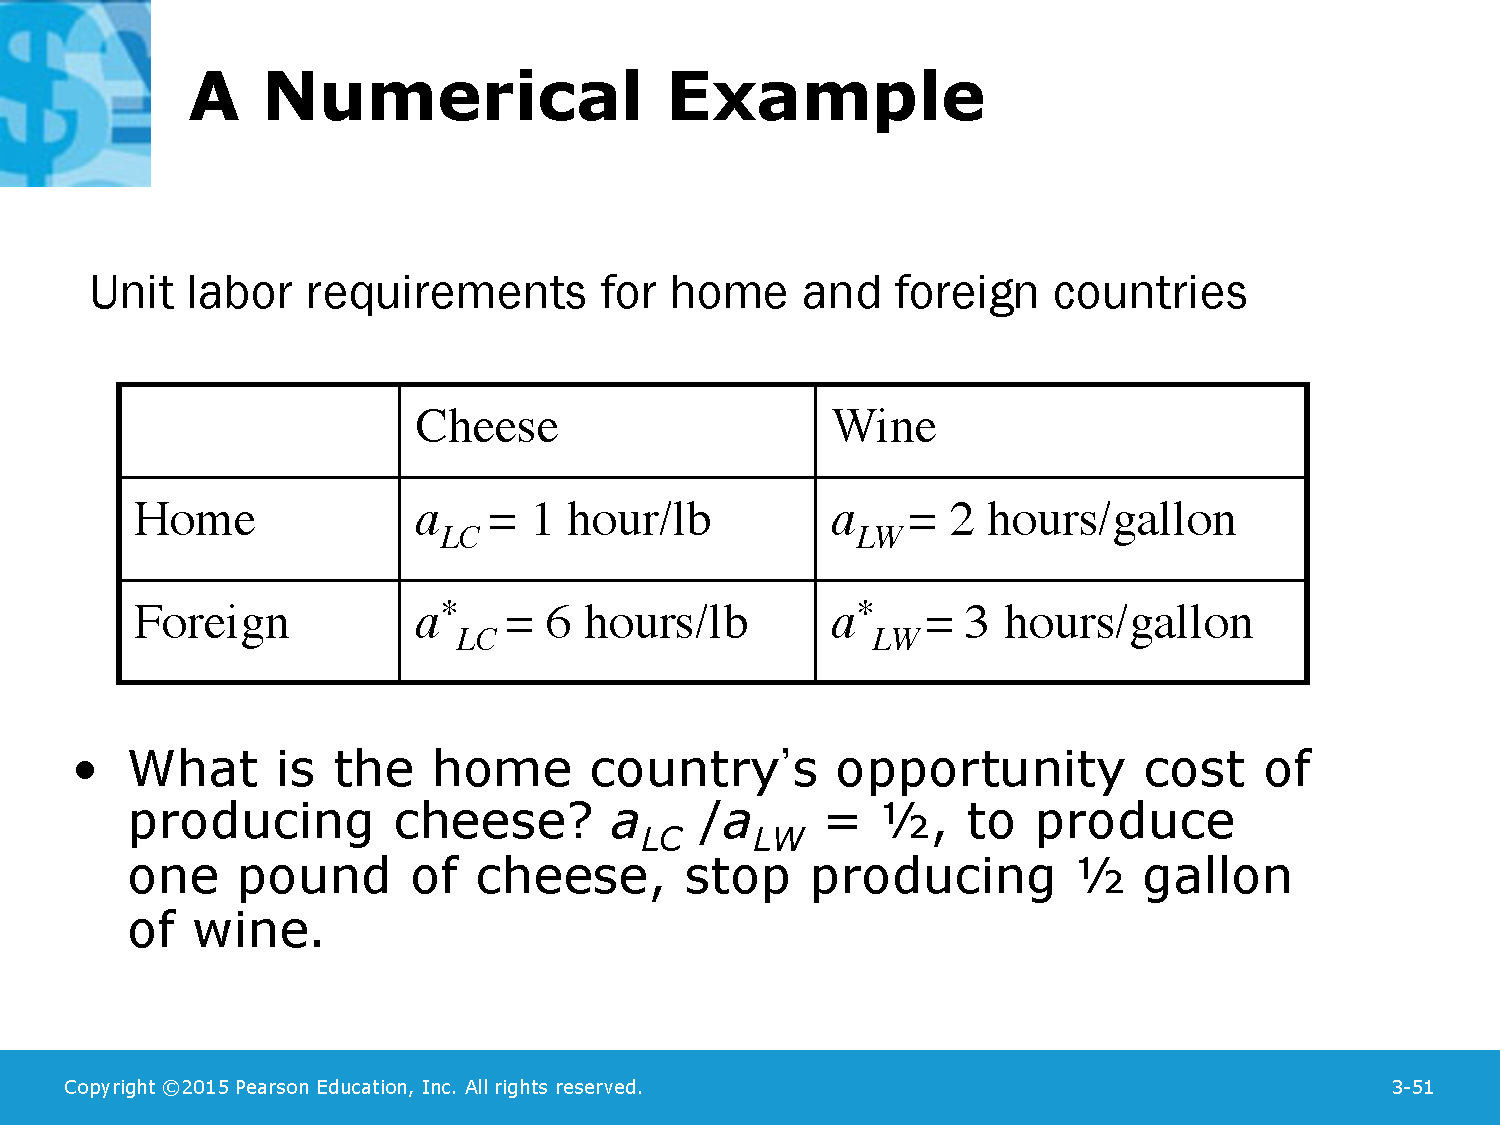
\includegraphics[page=1,width=\textwidth]{Numerical_example_pearson_snippet.pdf}}
\frame[plain]{\includegraphics[page=2,width=\textwidth]{Numerical_example_pearson_snippet.pdf}}
\frame[plain]{\includegraphics[page=3,width=\textwidth]{Numerical_example_pearson_snippet.pdf}}
\frame[plain]{\includegraphics[page=4,width=\textwidth]{Numerical_example_pearson_snippet.pdf}}
\frame[plain]{\includegraphics[page=5,width=\textwidth]{Numerical_example_pearson_snippet.pdf}}
\frame[plain]{\includegraphics[page=6,width=\textwidth]{Numerical_example_pearson_snippet.pdf}}
\frame[plain]{\includegraphics[page=7,width=\textwidth]{Numerical_example_pearson_snippet.pdf}}
\frame[plain]{\includegraphics[page=8,width=\textwidth]{Numerical_example_pearson_snippet.pdf}}
\frame[plain]{\includegraphics[page=9,width=\textwidth]{Numerical_example_pearson_snippet.pdf}}
\frame[plain]{\includegraphics[page=10,width=\textwidth]{Numerical_example_pearson_snippet.pdf}}


\end{document}



